\textit{kursiv afsnit}

\section{Projektets metode}
I dette projekt anvendes HTA-core modellen, hvilket afspejles i projektets metode. Målet med anvendelse af HTA-core modellen er at analysere og diskutere de essentielle problemstillinger ved QST, samt at præsentere resultaterne fundet ved analysen og diskussionen \citep{HTAcore}. Ydermere bidrager benyttelsen af HTA-core modellen til en systematisk og bred vurdering af QST. Dette giver et evidensbaseret grundlag til beslutningstagning i forhold til eventuel implementation af QST. \citep{metodehaandbogen} \citep{HTAcore} HTA-core modellen anvendes til besvarelse af problemformuleringen, da denne lægger op til en analyse af væsentlige faktorer ved QST, set ud fra et sundhedsvidenskabeligt perspektiv. Ved anvendelse af HTA-core inddeles analysen af teknologien i ni forskellige områder \citep{HTAcore}:

\begin{enumerate}
\item Sundhedsmæssigt problem og nuværende brug af teknologien (CUR)
\item Beskrivelse og tekniske karakteristika for teknologien (TEC)
\item Klinisk effekt (EFF)
\item Sikkerhed (SAF)
\item Organisatoriske aspekter (ORG)
\item Patient- og sociale aspekter (SOC)
\item Etisk analyse (ETH)
\item Juridiske aspekter (LEG)
\item Omkostninger og økonomisk evaluering (ECO)
\end{enumerate}

Benyttelsen af HTA-core modellen illustreres på \figref{fig:VORESMODEL}. I dette projekt er områderne opsat som det fremgår af rækkefølgen ovenover, men som det ses ud fra \figref{fig:metode}, er der et sammenspil mellem områderne. 

\begin{figure}[H] 
	\begin{center}
		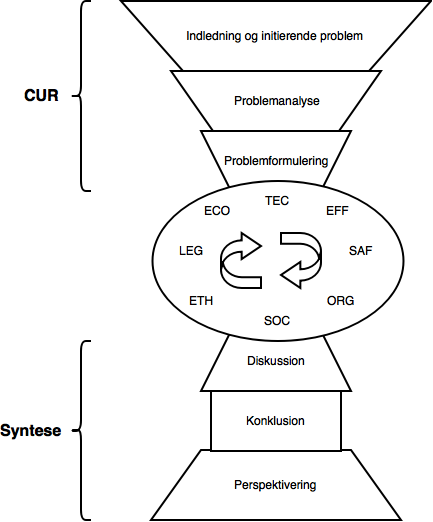
\includegraphics[width=0.5\textwidth]{figures/cMetode/metode}
	\end{center}
	\caption{VORES-model, der anvendes i projektet. Det ses, hvordan...} 
	\label{fig:metode} 
\end{figure}

Som det ses ud fra \figref{fig:metode} 
\textbf{Argument for overgangen mellem billedet her og næste afsnit om vurderingselementer}

Vurderingselementer er en betegnelse for det samlede produkt for analysen af et af de ni områder. Hvert domæne bliver inddelt i emner der hver skal klarlægge et bestemt problem indenfor området. Hvert emne specificeres yderligere ved konkrete HTA-spørgsmål, som skal besvares for at kunne besvare problemformuleringen. Når et eller flere HTA-spørgsmål under et emne er besvaret, kan besvarelsen af emnet samles med svar fra andre emner i domænet, i en delkonklusion. Delkonklusionen er besvarelsen af et domæne, og svaret indgår som et vurderingselement til den endelige besvarelse af problemformuleringen. \citep{HTAcore} \Figref{fig:vurderingselement} viser den beskrevne opbygning af vurderingselementet. 

\begin{figure}[H] 
\begin{center}
\includegraphics[width=0.5\textwidth]{figures/cMetode/vurderingselement}
\end{center}
\caption{Opbygningen af et vurderingselement. Figuren viser, hvordan vurderingselementet samlet er udgjort af de tre elementer; område, emne og problematik.}
\label{fig:vurderingselement} 
\end{figure}

I dette projekt opstilles analyseområderne med inspiration fra retningslinjerne i håndbogen for HTA-core modellen. Disse retningslinjer omfatter blandt andet hvilke emner, der bør afdækkes indenfor de enkelte domæner samt generelle forslag til spørgsmål. Det fremgår desuden, hvilke andre vurderingselementer, domænet relaterer til. Herudover angives det, hvilken metode og hvilken type litteratur, der kan være medvirkende til at besvare et givent domæne. \citep{HTAcore} \\
Afslutningsvis vil de enkelte vurderingselementer og problemformuleringen, sammenfattes i en syntese indeholdende en diskussion af resultater og en konklusion på problemformuleringen. 

\subsection{Argumentation for valg af domæner}
Før besvarelse af hvert domæne, argumenteres der for det enkelte domænes relevans for besvarelsen af problemformuleringen. Dette skal sikre at kun de vurderingselementer der bidrager til besvarelse af problemformuleringen besvares i projektet. 

Det første domæne, CUR, lægger op til analyse af et sundhedsmæssigt problem og mulige løsninger på problemet. Hermed er domænet relevant for dette projekt, idet det er gennem CUR-domænet det problem som resten af domænerne forsøger at besvare findes. CUR-domænet besvares ved benyttelsen af en AAU-inspireret tilgang. Først indledes projektet med et initierende problem, der lægger op til en bred, alsidig undersøgelse af relevante aspekter for projektet, hvilke undersøges i problemanalysen for at finde et konkret problem, som ønskes besvaret. Igennem analysen bliver det initierende problem undersøgt og afslutningsvis afgrænset, hvormed der kan opstilles en problemformulering. Problemformuleringen definerer det konkrete problem, og besvares igennem de resterende domæner i HTA-core modellen. De første to kapitler (\chapref{introduktion} og \chapref{problemanalyse}), udgør dermed i dette projekt CUR analysen. De resterende områders metode vil blive beskrevet i deres respektive analyser. 

I domænet TEC undersøges den valgte teknologi, både i forhold til oprindelige formål og hvordan teknologien kan anvendes i forhold til det opstillede problem. Idet QST er en gammel metode, som indeholder et stort spænd af protokoller er det relevant at inddrage TEC domænet, for at få et indgående kendskab til både den generelle QST og de QST-parametre som anvendes til undersøgelse af knæartrosepatienter. Ligeledes er et kendskab til QST, dennes krav til patienter og brugere samt mulighederne for samspillet mellem QST og klinikeren nødvendige før det er muligt at analysere flere af de andre domæner. 

Domænet EFF har til formål at analysere en teknologi ud fra dens effektivitet og virkningsgrad. Idet QST-undersøgelser af knæartrosepatienter er et relativt nyt tiltag, vil det være relevant at undersøge hvor effektive disse undersøgelser er i forhold til sensitivitet og specificitet. Dette domæne er ligeledes en relevant del af projektet idet overvejelser fra området kan inddrages i eksempelvis ECO-området.   


Ved SAF-området undersøges sikkerhedsrisici ved en teknologi. Ved QST-undersøgelser tilpasset kroniske postoperative smerter tilføres en patient smerte for at vurdere patientens reaktion ud fra forskellige parametre. Hermed kan der være sikkerhedsmæssige risici for patienten, hvilket kan føre til eventuelle skader. Det er dermed relevant at undersøge om de undersøgelsesmetoder der anvendes i QST kan skade patienten samt i hvilket omfang dette kan ske. Dette gør det muligt at vurdere hvorvidt de sikkerhedsmæssige risici ved QST-undersøgelserne overgår den diagnostiske relevans for undersøgelserne. 

\textbf{ORG}

\textbf{SOC}

Ved ETH-domænet undersøges de etiske aspekter ved en teknologi. Da QST skal anvendes som vurderingsgrundlag forud for en operation vil det have etiske konsekvenser, hvis QST ikke kan identificere alle patienter med forhøjet risiko for udvikling af kroniske postoperative smerter. Disse overvejelser vil både gælde for falsk positive og falsk negative resultater. \textbf{Tilføj hvad end er besluttes ift nye spørgsmål}       

\textbf{LEG}

I ECO-domænet undersøges problemet ud fra et økonomisk synspunkt. Da det for QST-undersøgelserne er nødvendigt at anvende teknologisk udstyr, er der omkostninger forbundet med implementering af disse. Ligeledes vil der blandt andet være omkostninger ved oplæring af personale. Disse økonomiske omkostninger sættes op imod gevinster ved implementeringen af QST. Disse gevinster kan være både monetære eller tage anden form. Det er relevant at undersøge implementeringen og brugen af QST ud fra et økonomisk perspektiv, idet dette er en betydelig del af et politisk vurderingsgrundlag. 

\subsection{Litteratursøgning} \label{sec_lit}
Litteratursøgning og -vurdering i projektet tager udgangspunkt i retningslinjerne opstillet i Metodehåndbogen for Medicinsk Teknologivurdering udarbejdet af Sundhedsstyrelsen \citep{metodehaandbogen}. Da projektet udarbejdes på baggrund af videnskabelig litteratur, er det væsentligt, at litteraturen findes og vurderes ved en organiseret fremgangsmåde, således at problemformuleringen besvares på et veldokumenteret grundlag. Litteratursøgningen vil derfor være den samme for alle områder af rapporten. For hvert domænes metode vil litteratursøgning kun beskrives i så fald søgningen for det specifikke område afviger fra den generelle litteratursøgningsmetode som beskrevet her. \\
Generelt for litteratursøgning vil der blive søgt på sundhedsvidenskabelige databaser som: PubMed, MEDLINE, EMBASE og Cochrane Library. Aalborg Universitetsbiblioteks søgemaskine Primo vil ligeledes tages i brug og anvendes som generel søgeværktøj, da denne dækker mange databaser. For ligeledes at sikre ensartethed gennem rapporten vil udvælgelsen og vurderingen af litteratur forløbe efter samme søgestrategi for alle områder. 

Litteratur er søgt således, at antal hits per søgning, befinder sig ~100. Dette betyder at alle overskrifter for den pågældende søgning er blevet gennemgået for relevans. Ved de udvalgte artikler, er abstract efterfølgende blevet gennemlæst for at sortere materialet. De artikler som er blevet fundet relevante til besvarelse af HTA-spørgsmålet, er blevet kritisk gennemgået. Ved enkelte artikler er snowballing blevet benyttet. Her gennemlæses fundne studiers referenceliste og relevante studier herfra anvendes til besvarelse af HTA-spørgsmålet.

Søgeprotokollen har ligeledes til formål at gøre det muligt for interessenter at forstå, hvordan litteratursøgningen er forløbet. \citep{metodehaandbogen} Til at udarbejde søgeprotokollen i dette projekt, er der opstillet en skabelon, der systematiserer litteratursøgningen. Et uddrag af skabelonen ses i \figref{fig:soegeprotokol}.

\begin{figure}[H]
\begin{center}

\includegraphics[width=0.5\textwidth]{figures/cMetode/soegeprotokol}
\end{center}
\caption{Skabelon for projektets søgeprotokol. Det fremgår af skabelonen, at der for hver søgning skal opstilles ét HTA-spørgsmål samt inklusions- og eksklusionskriterier. Det skal ligeledes dokumenteres, hvilke databaser, der er anvendt til søgningen. For hver database skal de specifikt anvendte søgeord opstilles, og antallet hits skal efterfølgende fremgå.}
\label{fig:soegeprotokol} 
\end{figure}

HTA-spørgsmålet i søgeprotokollen har til formål at bidrage til besvarelsen af problemformuleringen indenfor de otte domæner. Spørgsmålene skal være helt afgrænsede og entydige, således at det er muligt at finde konkret litteratur, og besvare dem præcist. \citep{metodehaandbogen}  
For at afgrænse og sikre relevansen af søgeresultaterne, opstilles inklusions- og eksklusionskriterier for søgningerne. Søgningerne kan eksempelvis afgrænses til kun at indeholde bestemte typer studier, en eller få specifikke sygdomme, en afgrænset aldersgruppe med mere. \citep{metodehaandbogen} \\
Dokumentationen af valgte databaser samt tilhørende specifikke søgeord er en væsentlig del af søgeprotokollen, da databaserne har forskellige typer syntaks til litteratursøgning, hvormed det er vigtigt, at søgningen i en given database er foretaget med anvendelse af søgetermerne specifikke for den valgte database. \citep{metodehaandbogen}
Efter litteratursøgningen vurderes den fundne litteratur med henblik på at udvælge de kilder, der bedst kan besvare de fokuserede spørgsmål og dermed den overordnede problemstilling for projektet. Det er således essentielt at kontrollere, om det, der undersøges i udvalgt litteratur, har relevans for de fokuserede spørgsmål eksempelvis ved gennemlæsning af abstract, metode samt resultater. Ligeledes vurderes studiers evidensniveau, for at sikre kvaliteten af besvarelserne. \citep{metodehaandbogen} 
Litteraturen i dette projekt inddeles ud fra evidenshierakiet i \citer{metodehaandbogen}. Evidenshierakiet omfatter følgende syv punkter, hvor kilder med det højeste evidensniveau er placeret øverst i listen:

\begin{enumerate}
\item Metaanalyser og systematiske undersøgelser 
\item Randomiserede kontrollerede undersøgelser (RCT’s)
\item Ikke-randomiserede kontrollerede undersøgelser
\item Kohorte undersøgelser
\item Case-kontrol undersøgelser
\item Deskriptive undersøgelser, mindre serier
\item Konsensusrapporter, ikke-systematiske oversigtsartikler, ledere, ekspertudtalelser
\end{enumerate}

Metaanalyser og systematiske undersøgelser er sekundær litteratur og har det højeste evidensniveau. Denne type litteratur er statiske sammenfatninger af primær litteratur med samme afgrænsede problemstilling. \citep{denstoredanske2009} \\
Randomiserede kontrollerede undersøgelser (RCT) er primær litteratur, hvor der foretages en sammenligning af to forsøgsgrupper. Den ene gruppe udsættes for en påvirkning, mens den anden gruppe fungerer som kontrolgruppe. Udvælgelsen af forsøgspersoner foregår tilfældigt. \citep{denstoredanske2009a} \\
Ikke-randomiserede kontrollerede undersøgelser er ligesom RCT’s primær litteratur, hvor to forsøgsgrupper sammenlignes. Ved disse undersøgelser sker udvælgelsen af forsøgspersoner ikke tilfældigt, hvormed evidensniveauet falder da der ikke på samme måde som ved RCT tages højde for bias i forsøgsgrupperne. \citep{denstoredanske2009a} \\
Ved kohorte undersøgelser følges flere forsøgsgrupper over en periode for at undersøge, hvorvidt bestemte eksponeringer har indflydelse på udviklingen af helbredsfænomener, herunder sygdom og død. \citep{metodehaandbogen} \\
I case-kontrol undersøgelser, forsøges det at undersøge forskellige faktorers indflydelse på udvikling af bestemte sygdomme. Dette gøres ved en sammenligning mellem en forsøgsgruppe med den pågældende sygdom og en forsøgsgruppe bestående af raske personer. I modsætning til eksempelvis kohortestudiet følges forsøgsgrupperne ikke over tid, hvormed der ikke kan udføres en opfølgende undersøgelse. Det er således ikke muligt at estimere betydningen af  risikofaktorerne. \citep{denstoredanske2012} \\
Deskriptive studier er studier hvor der foretages analyser til beskrivelse af et fænomen. I modsætning til de andre typer studier påvirkes forsøgsgrupperne ikke. I stedet undersøges nuværende tendenser, eksempelvis med henblik på senere udførelse af et forsøg. \citep{} \\
Fælles for gruppen af konsensusrapporter, ikke-systematiske oversigtsartikler samt ledere og ekspertudtalelser er, at materialet oftest er udtryk for subjektive holdninger, der ikke er underbygget af tilstrækkelige mængder supplerende litteratur, der undersøger området. \citep{metodehaandbogen}  